% Options for packages loaded elsewhere
\PassOptionsToPackage{unicode}{hyperref}
\PassOptionsToPackage{hyphens}{url}
%
\documentclass[
]{article}
\usepackage{amsmath,amssymb}
\usepackage{iftex}
\ifPDFTeX
  \usepackage[T1]{fontenc}
  \usepackage[utf8]{inputenc}
  \usepackage{textcomp} % provide euro and other symbols
\else % if luatex or xetex
  \usepackage{unicode-math} % this also loads fontspec
  \defaultfontfeatures{Scale=MatchLowercase}
  \defaultfontfeatures[\rmfamily]{Ligatures=TeX,Scale=1}
\fi
\usepackage{lmodern}
\ifPDFTeX\else
  % xetex/luatex font selection
\fi
% Use upquote if available, for straight quotes in verbatim environments
\IfFileExists{upquote.sty}{\usepackage{upquote}}{}
\IfFileExists{microtype.sty}{% use microtype if available
  \usepackage[]{microtype}
  \UseMicrotypeSet[protrusion]{basicmath} % disable protrusion for tt fonts
}{}
\makeatletter
\@ifundefined{KOMAClassName}{% if non-KOMA class
  \IfFileExists{parskip.sty}{%
    \usepackage{parskip}
  }{% else
    \setlength{\parindent}{0pt}
    \setlength{\parskip}{6pt plus 2pt minus 1pt}}
}{% if KOMA class
  \KOMAoptions{parskip=half}}
\makeatother
\usepackage{xcolor}
\usepackage[margin=1in]{geometry}
\usepackage{color}
\usepackage{fancyvrb}
\newcommand{\VerbBar}{|}
\newcommand{\VERB}{\Verb[commandchars=\\\{\}]}
\DefineVerbatimEnvironment{Highlighting}{Verbatim}{commandchars=\\\{\}}
% Add ',fontsize=\small' for more characters per line
\usepackage{framed}
\definecolor{shadecolor}{RGB}{248,248,248}
\newenvironment{Shaded}{\begin{snugshade}}{\end{snugshade}}
\newcommand{\AlertTok}[1]{\textcolor[rgb]{0.94,0.16,0.16}{#1}}
\newcommand{\AnnotationTok}[1]{\textcolor[rgb]{0.56,0.35,0.01}{\textbf{\textit{#1}}}}
\newcommand{\AttributeTok}[1]{\textcolor[rgb]{0.13,0.29,0.53}{#1}}
\newcommand{\BaseNTok}[1]{\textcolor[rgb]{0.00,0.00,0.81}{#1}}
\newcommand{\BuiltInTok}[1]{#1}
\newcommand{\CharTok}[1]{\textcolor[rgb]{0.31,0.60,0.02}{#1}}
\newcommand{\CommentTok}[1]{\textcolor[rgb]{0.56,0.35,0.01}{\textit{#1}}}
\newcommand{\CommentVarTok}[1]{\textcolor[rgb]{0.56,0.35,0.01}{\textbf{\textit{#1}}}}
\newcommand{\ConstantTok}[1]{\textcolor[rgb]{0.56,0.35,0.01}{#1}}
\newcommand{\ControlFlowTok}[1]{\textcolor[rgb]{0.13,0.29,0.53}{\textbf{#1}}}
\newcommand{\DataTypeTok}[1]{\textcolor[rgb]{0.13,0.29,0.53}{#1}}
\newcommand{\DecValTok}[1]{\textcolor[rgb]{0.00,0.00,0.81}{#1}}
\newcommand{\DocumentationTok}[1]{\textcolor[rgb]{0.56,0.35,0.01}{\textbf{\textit{#1}}}}
\newcommand{\ErrorTok}[1]{\textcolor[rgb]{0.64,0.00,0.00}{\textbf{#1}}}
\newcommand{\ExtensionTok}[1]{#1}
\newcommand{\FloatTok}[1]{\textcolor[rgb]{0.00,0.00,0.81}{#1}}
\newcommand{\FunctionTok}[1]{\textcolor[rgb]{0.13,0.29,0.53}{\textbf{#1}}}
\newcommand{\ImportTok}[1]{#1}
\newcommand{\InformationTok}[1]{\textcolor[rgb]{0.56,0.35,0.01}{\textbf{\textit{#1}}}}
\newcommand{\KeywordTok}[1]{\textcolor[rgb]{0.13,0.29,0.53}{\textbf{#1}}}
\newcommand{\NormalTok}[1]{#1}
\newcommand{\OperatorTok}[1]{\textcolor[rgb]{0.81,0.36,0.00}{\textbf{#1}}}
\newcommand{\OtherTok}[1]{\textcolor[rgb]{0.56,0.35,0.01}{#1}}
\newcommand{\PreprocessorTok}[1]{\textcolor[rgb]{0.56,0.35,0.01}{\textit{#1}}}
\newcommand{\RegionMarkerTok}[1]{#1}
\newcommand{\SpecialCharTok}[1]{\textcolor[rgb]{0.81,0.36,0.00}{\textbf{#1}}}
\newcommand{\SpecialStringTok}[1]{\textcolor[rgb]{0.31,0.60,0.02}{#1}}
\newcommand{\StringTok}[1]{\textcolor[rgb]{0.31,0.60,0.02}{#1}}
\newcommand{\VariableTok}[1]{\textcolor[rgb]{0.00,0.00,0.00}{#1}}
\newcommand{\VerbatimStringTok}[1]{\textcolor[rgb]{0.31,0.60,0.02}{#1}}
\newcommand{\WarningTok}[1]{\textcolor[rgb]{0.56,0.35,0.01}{\textbf{\textit{#1}}}}
\usepackage{graphicx}
\makeatletter
\def\maxwidth{\ifdim\Gin@nat@width>\linewidth\linewidth\else\Gin@nat@width\fi}
\def\maxheight{\ifdim\Gin@nat@height>\textheight\textheight\else\Gin@nat@height\fi}
\makeatother
% Scale images if necessary, so that they will not overflow the page
% margins by default, and it is still possible to overwrite the defaults
% using explicit options in \includegraphics[width, height, ...]{}
\setkeys{Gin}{width=\maxwidth,height=\maxheight,keepaspectratio}
% Set default figure placement to htbp
\makeatletter
\def\fps@figure{htbp}
\makeatother
\setlength{\emergencystretch}{3em} % prevent overfull lines
\providecommand{\tightlist}{%
  \setlength{\itemsep}{0pt}\setlength{\parskip}{0pt}}
\setcounter{secnumdepth}{-\maxdimen} % remove section numbering
\ifLuaTeX
  \usepackage{selnolig}  % disable illegal ligatures
\fi
\usepackage{bookmark}
\IfFileExists{xurl.sty}{\usepackage{xurl}}{} % add URL line breaks if available
\urlstyle{same}
\hypersetup{
  pdftitle={Project Network-based Data Analysis},
  pdfauthor={Annalisa Xamin},
  hidelinks,
  pdfcreator={LaTeX via pandoc}}

\title{Project Network-based Data Analysis}
\author{Annalisa Xamin}
\date{}

\begin{document}
\maketitle

{
\setcounter{tocdepth}{2}
\tableofcontents
}
\begin{center}\rule{0.5\linewidth}{0.5pt}\end{center}

\subsection{Install and load R
packages}\label{install-and-load-r-packages}

\begin{Shaded}
\begin{Highlighting}[]
\ControlFlowTok{if}\NormalTok{ (}\SpecialCharTok{!}\FunctionTok{require}\NormalTok{(}\StringTok{"BiocManager"}\NormalTok{, }\AttributeTok{quietly =} \ConstantTok{TRUE}\NormalTok{))}
    \FunctionTok{install.packages}\NormalTok{(}\StringTok{"BiocManager"}\NormalTok{)}

\ControlFlowTok{if}\NormalTok{ (}\SpecialCharTok{!}\FunctionTok{require}\NormalTok{(}\StringTok{"GEOquery"}\NormalTok{, }\AttributeTok{quietly =} \ConstantTok{TRUE}\NormalTok{))}
\NormalTok{    BiocManager}\SpecialCharTok{::}\FunctionTok{install}\NormalTok{(}\StringTok{"GEOquery"}\NormalTok{) }

\ControlFlowTok{if}\NormalTok{ (}\SpecialCharTok{!}\FunctionTok{require}\NormalTok{(}\StringTok{"rScudo"}\NormalTok{, }\AttributeTok{quietly =} \ConstantTok{TRUE}\NormalTok{))}
\NormalTok{    BiocManager}\SpecialCharTok{::}\FunctionTok{install}\NormalTok{(}\StringTok{"rScudo"}\NormalTok{) }

\FunctionTok{library}\NormalTok{(tidyverse)}
\FunctionTok{library}\NormalTok{(dplyr)}
\FunctionTok{library}\NormalTok{(GEOquery)}
\FunctionTok{library}\NormalTok{(rScudo)}
\FunctionTok{library}\NormalTok{(plotly)}
\end{Highlighting}
\end{Shaded}

\section{Data selection}\label{data-selection}

The analysis will use the dataset
\href{https://www.ncbi.nlm.nih.gov/geo/query/acc.cgi?acc=GSE20437}{GSE20437}
obtained from GEO.The dataset is generated from Affymetrix HU133A
microarrays and contains 42 tissue samples.

In detail, the data includes:

\begin{itemize}
\item
  18 reduction mammoplasty (RM) breast epithelium samples,
\item
  18 histologically normal (HN) epithelial samples from breast cancer
  patients (9 ER+ and 9 ER-), and
\item
  6 histologically normal epithelial samples from prophylactic
  mastectomy patients.
\end{itemize}

Note that sample numbers correspond to individual patient samples.

\begin{Shaded}
\begin{Highlighting}[]
\CommentTok{\# download the GSE20437 expression data series}
\NormalTok{gse }\OtherTok{\textless{}{-}} \FunctionTok{getGEO}\NormalTok{(}\StringTok{"GSE20437"}\NormalTok{, }\AttributeTok{destdir=} \StringTok{\textquotesingle{}./data/\textquotesingle{}}\NormalTok{, }\AttributeTok{getGPL =}\NormalTok{ F)}
\end{Highlighting}
\end{Shaded}

\begin{verbatim}
## Found 1 file(s)
\end{verbatim}

\begin{verbatim}
## GSE20437_series_matrix.txt.gz
\end{verbatim}

\begin{verbatim}
## Using locally cached version: ./data//GSE20437_series_matrix.txt.gz
\end{verbatim}

\begin{Shaded}
\begin{Highlighting}[]
\CommentTok{\# getGEO returns a list of expression objects, but...}
\FunctionTok{length}\NormalTok{(gse) }
\end{Highlighting}
\end{Shaded}

\begin{verbatim}
## [1] 1
\end{verbatim}

\begin{Shaded}
\begin{Highlighting}[]
\CommentTok{\# shows us there is only one object in it. }
\CommentTok{\# We assign it to the same variable.}
\NormalTok{gse }\OtherTok{\textless{}{-}}\NormalTok{ gse[[}\DecValTok{1}\NormalTok{]]}
\end{Highlighting}
\end{Shaded}

\section{Exploratory analysis}\label{exploratory-analysis}

\begin{Shaded}
\begin{Highlighting}[]
\CommentTok{\# show what we have:}
\FunctionTok{show}\NormalTok{(gse)}
\end{Highlighting}
\end{Shaded}

\begin{verbatim}
## ExpressionSet (storageMode: lockedEnvironment)
## assayData: 22283 features, 42 samples 
##   element names: exprs 
## protocolData: none
## phenoData
##   sampleNames: GSM512539 GSM512540 ... GSM512580 (42 total)
##   varLabels: title geo_accession ... tissue:ch1 (38 total)
##   varMetadata: labelDescription
## featureData: none
## experimentData: use 'experimentData(object)'
##   pubMedIds: 20197764 
## Annotation: GPL96
\end{verbatim}

The actual expression data are accessible in the \texttt{exprs} section
of \texttt{gse}, an Expression Set and the generic data class that
BioConductor uses for expression data.

\begin{Shaded}
\begin{Highlighting}[]
\FunctionTok{head}\NormalTok{(}\FunctionTok{exprs}\NormalTok{(gse)) }
\end{Highlighting}
\end{Shaded}

\begin{verbatim}
##           GSM512539 GSM512540 GSM512541 GSM512542 GSM512543 GSM512544 GSM512545
## 1007_s_at    2461.4    3435.7    1932.5    2377.7    3055.3    2978.1    2348.5
## 1053_at        26.7     159.0      31.2     140.7      69.9      98.5      37.0
## 117_at         82.6     243.4     150.2      95.1     209.3     103.4      91.2
## 121_at        942.3     897.5     840.8     870.9     685.4     791.8     886.5
## 1255_g_at      71.8      87.9      75.4      58.1      31.8      40.3      70.5
## 1294_at       630.2     571.4     346.3     679.9    1289.3     421.1     417.6
##           GSM512546 GSM512547 GSM512548 GSM512549 GSM512550 GSM512551 GSM512552
## 1007_s_at    2963.9    2776.9    3088.9    3033.3    3037.1    3545.8    3322.6
## 1053_at        59.9      86.7     107.2      64.0      82.9      97.7      69.7
## 117_at        168.4     162.7     203.2     143.7     113.5      80.0     186.4
## 121_at        954.2     843.1     775.3     847.6     912.2     911.6     862.4
## 1255_g_at      43.3      51.6      42.6      74.9      53.7      30.5      15.2
## 1294_at       811.6     778.1     393.2     995.4     987.7     938.5     924.6
##           GSM512553 GSM512554 GSM512555 GSM512556 GSM512557 GSM512558 GSM512559
## 1007_s_at    1963.7    3609.6    2078.9    4138.6    4260.7    2453.6    2709.0
## 1053_at        82.0      45.6      84.5      31.7      37.4      82.4     204.8
## 117_at        106.6     145.6     144.4     133.6     278.6     173.0     147.8
## 121_at        705.0     984.6     853.8     846.8    1273.0     833.6     908.1
## 1255_g_at      42.5      76.6      88.2      90.6      65.8      25.8      77.5
## 1294_at       480.8    1054.1     632.0     448.0    1345.2    1248.9     405.7
##           GSM512560 GSM512561 GSM512562 GSM512563 GSM512564 GSM512565 GSM512566
## 1007_s_at    2612.5    4340.1    3155.3    2390.3    2738.8    3233.1    2836.6
## 1053_at       119.3      76.7     100.3     115.4      14.1      47.6      77.1
## 117_at        186.0     168.0      95.2      73.6     122.7     107.6     120.9
## 121_at        806.2     827.0     629.4     709.2     305.6     877.4     425.7
## 1255_g_at      84.3      87.9      44.6      59.3      12.0      82.1      59.2
## 1294_at       647.5    2218.1    1321.1     606.7    1709.9     980.8    1268.4
##           GSM512567 GSM512568 GSM512569 GSM512570 GSM512571 GSM512572 GSM512573
## 1007_s_at    2915.4    3457.5    2798.7    4370.2    2467.3    3669.5    3310.1
## 1053_at        47.1      47.0      83.2      40.2      80.3      24.1       8.8
## 117_at        143.4      92.5      72.1     131.8     156.4     165.8     141.6
## 121_at        643.8     771.3     681.1     812.7     533.4     746.9    1090.3
## 1255_g_at      62.2      28.3      97.6       8.1      17.9      53.0      39.9
## 1294_at       955.8    1157.5     888.6    1130.8     905.1    1138.5     483.0
##           GSM512574 GSM512575 GSM512576 GSM512577 GSM512578 GSM512579 GSM512580
## 1007_s_at    3942.2    4520.4    3596.1    2989.0    3164.5    2764.3    4258.5
## 1053_at        44.6      54.7      56.7      89.9      63.4      57.0      59.5
## 117_at         97.1     132.7     124.3     210.5     131.4      89.6     123.3
## 121_at       1008.7     718.6     988.4     295.9     957.3     630.8     869.2
## 1255_g_at      11.0      50.2      60.0      34.3      33.5      61.7      50.4
## 1294_at      1326.5    1179.4     668.3     863.2    1055.5    1287.6    1127.8
\end{verbatim}

To conveniently access the data rows and columns present in
\texttt{exprs(gse)}, this matrix is assigned to its own variable
\texttt{ex}.

\begin{Shaded}
\begin{Highlighting}[]
\CommentTok{\# exprs (gse) is a matrix that we can assign to its own variable, to}
\CommentTok{\# conveniently access the data rows and columns}
\NormalTok{ex }\OtherTok{\textless{}{-}} \FunctionTok{exprs}\NormalTok{(gse)}
\FunctionTok{dim}\NormalTok{(ex) }\CommentTok{\# 42 sample, 22283 genes}
\end{Highlighting}
\end{Shaded}

\begin{verbatim}
## [1] 22283    42
\end{verbatim}

The dataset contains gene expression data of 22283 genes (rows) from 42
patients (columns).

\subsection{Pre-processing}\label{pre-processing}

\begin{Shaded}
\begin{Highlighting}[]
\CommentTok{\# Analyze value distributions}
\CommentTok{\#boxplot(ex)}
\FunctionTok{boxplot}\NormalTok{(ex, }\AttributeTok{main =} \StringTok{\textquotesingle{}Boxplot of the data before normalization\textquotesingle{}}\NormalTok{)}
\end{Highlighting}
\end{Shaded}

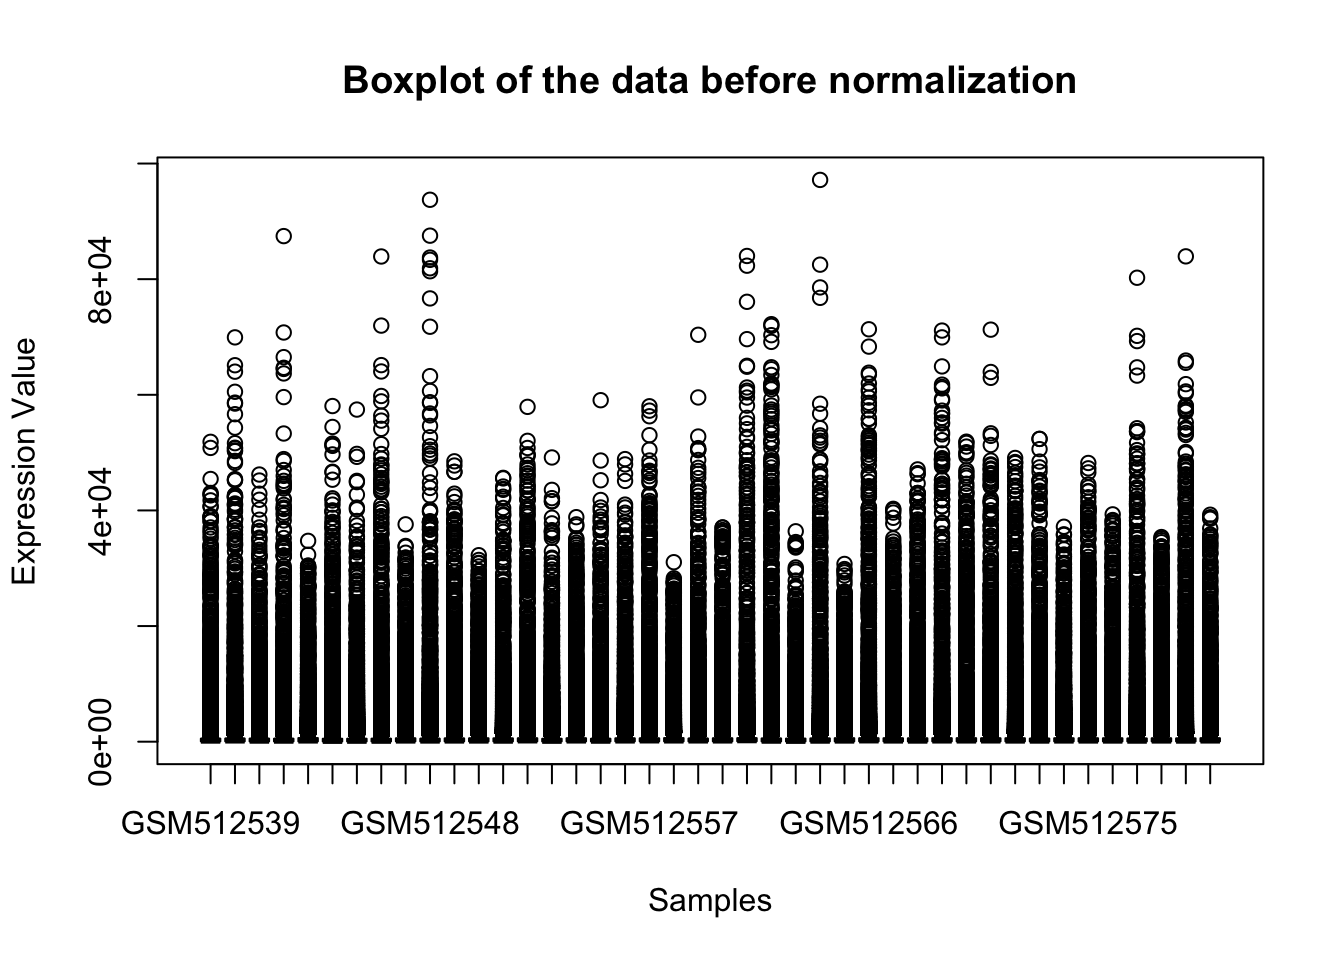
\includegraphics{NBDA_project_files/figure-latex/boxplot original data-1.pdf}

I try to apply a log transformation to the data to obtain a boxplot
easier to read.

\begin{Shaded}
\begin{Highlighting}[]
\NormalTok{ex2}\OtherTok{\textless{}{-}}\FunctionTok{log}\NormalTok{(ex)}
\NormalTok{ex2 }\OtherTok{\textless{}{-}} \FunctionTok{na.omit}\NormalTok{(}\FunctionTok{as.matrix}\NormalTok{(ex2))}
\FunctionTok{boxplot}\NormalTok{(ex2, }\AttributeTok{main =} \StringTok{\textquotesingle{}Boxplot of the data after applying a logarithmic transformation\textquotesingle{}}\NormalTok{)}
\end{Highlighting}
\end{Shaded}

\begin{figure}
\centering
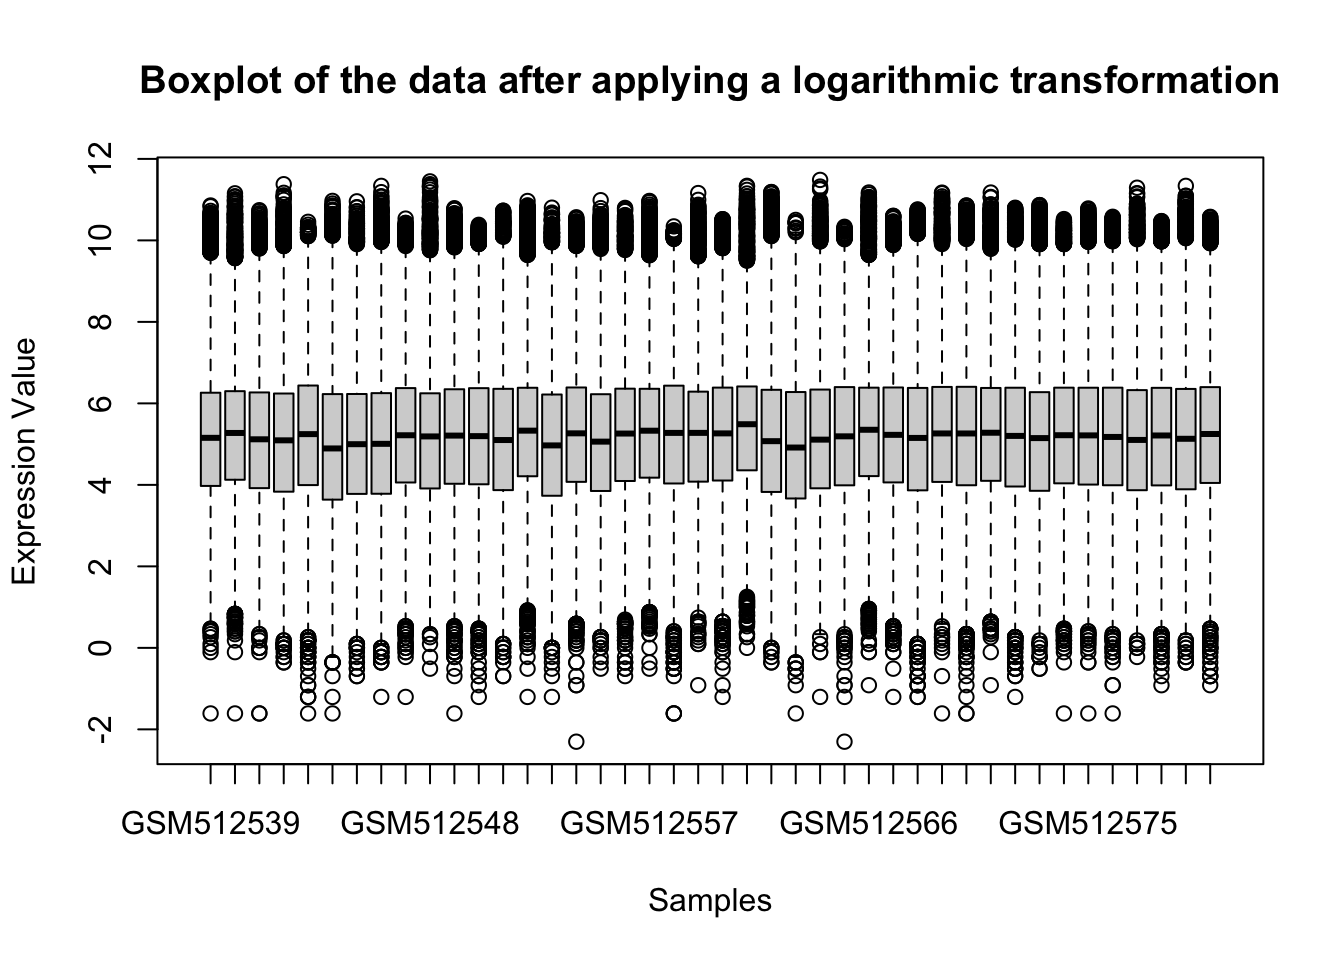
\includegraphics{NBDA_project_files/figure-latex/boxplot log transformation-1.pdf}
\caption{Boxplot of the data after applying a logarithmic
transformation}
\end{figure}

From the boxplot after the log transformation, I can see that there is
some variation in the median of the samples. So, I try to apply a median
normalization to the data after the log transformation.

\begin{Shaded}
\begin{Highlighting}[]
\CommentTok{\# MEDIAN NORMALIZATION}
\NormalTok{channel.medians}\OtherTok{=}\FunctionTok{apply}\NormalTok{(}\FunctionTok{log}\NormalTok{(ex),}\DecValTok{2}\NormalTok{,median)}
\NormalTok{normalized.log.ex}\OtherTok{=}\FunctionTok{sweep}\NormalTok{(}\FunctionTok{log}\NormalTok{(ex),}\DecValTok{2}\NormalTok{,channel.medians,}\StringTok{"{-}"}\NormalTok{)}

\CommentTok{\# boxplot post median normalization on ex}
\FunctionTok{boxplot}\NormalTok{(normalized.log.ex, }\AttributeTok{main =} \StringTok{\textquotesingle{}Boxplot of the data after median normalization\textquotesingle{}}\NormalTok{)}
\end{Highlighting}
\end{Shaded}

\begin{figure}
\centering
\includegraphics{NBDA_project_files/figure-latex/median normalization and boxplot-1.pdf}
\caption{Boxplot of the data after median normalization}
\end{figure}

\subsection{PCA}\label{pca}

\begin{Shaded}
\begin{Highlighting}[]
\NormalTok{pca }\OtherTok{\textless{}{-}} \FunctionTok{prcomp}\NormalTok{(}\FunctionTok{t}\NormalTok{(normalized.log.ex))}
\FunctionTok{summary}\NormalTok{(pca) }\CommentTok{\# get the summary of the PCA, we get a table in which each column is a principal components and we have information on the standard deviation and the variation, etc}
\end{Highlighting}
\end{Shaded}

\begin{verbatim}
## Importance of components:
##                            PC1      PC2      PC3      PC4      PC5      PC6
## Standard deviation     38.8020 23.47065 20.63892 19.54327 18.43330 15.97431
## Proportion of Variance  0.1791  0.06552  0.05067  0.04543  0.04042  0.03035
## Cumulative Proportion   0.1791  0.24461  0.29527  0.34070  0.38112  0.41147
##                             PC7      PC8      PC9     PC10     PC11     PC12
## Standard deviation     15.54787 15.25339 14.95988 13.82648 13.67761 13.63388
## Proportion of Variance  0.02875  0.02767  0.02662  0.02274  0.02225  0.02211
## Cumulative Proportion   0.44023  0.46790  0.49452  0.51726  0.53951  0.56162
##                            PC13     PC14     PC15     PC16     PC17     PC18
## Standard deviation     13.39954 13.05683 12.96288 12.78929 12.64910 12.48152
## Proportion of Variance  0.02136  0.02028  0.01999  0.01946  0.01903  0.01853
## Cumulative Proportion   0.58298  0.60326  0.62324  0.64270  0.66173  0.68026
##                            PC19     PC20     PC21     PC22     PC23     PC24
## Standard deviation     12.32645 12.13869 12.04722 11.97088 11.90374 11.69483
## Proportion of Variance  0.01807  0.01753  0.01726  0.01705  0.01685  0.01627
## Cumulative Proportion   0.69833  0.71586  0.73312  0.75017  0.76702  0.78329
##                            PC25     PC26     PC27     PC28     PC29     PC30
## Standard deviation     11.60734 11.57222 11.46507 11.15870 11.04915 10.99769
## Proportion of Variance  0.01603  0.01593  0.01564  0.01481  0.01452  0.01439
## Cumulative Proportion   0.79932  0.81525  0.83088  0.84569  0.86021  0.87460
##                            PC31     PC32     PC33     PC34   PC35    PC36
## Standard deviation     10.68517 10.45191 10.25430 10.13818 9.9583 9.68456
## Proportion of Variance  0.01358  0.01299  0.01251  0.01223 0.0118 0.01116
## Cumulative Proportion   0.88818  0.90117  0.91368  0.92591 0.9377 0.94886
##                           PC37    PC38   PC39    PC40    PC41      PC42
## Standard deviation     9.50070 9.42259 9.3053 9.17335 8.95347 6.784e-14
## Proportion of Variance 0.01074 0.01056 0.0103 0.01001 0.00954 0.000e+00
## Cumulative Proportion  0.95960 0.97016 0.9805 0.99046 1.00000 1.000e+00
\end{verbatim}

\begin{Shaded}
\begin{Highlighting}[]
\FunctionTok{screeplot}\NormalTok{(pca) }\CommentTok{\# this plot show the variance explained by the first 10 components}
\end{Highlighting}
\end{Shaded}

\begin{figure}
\centering
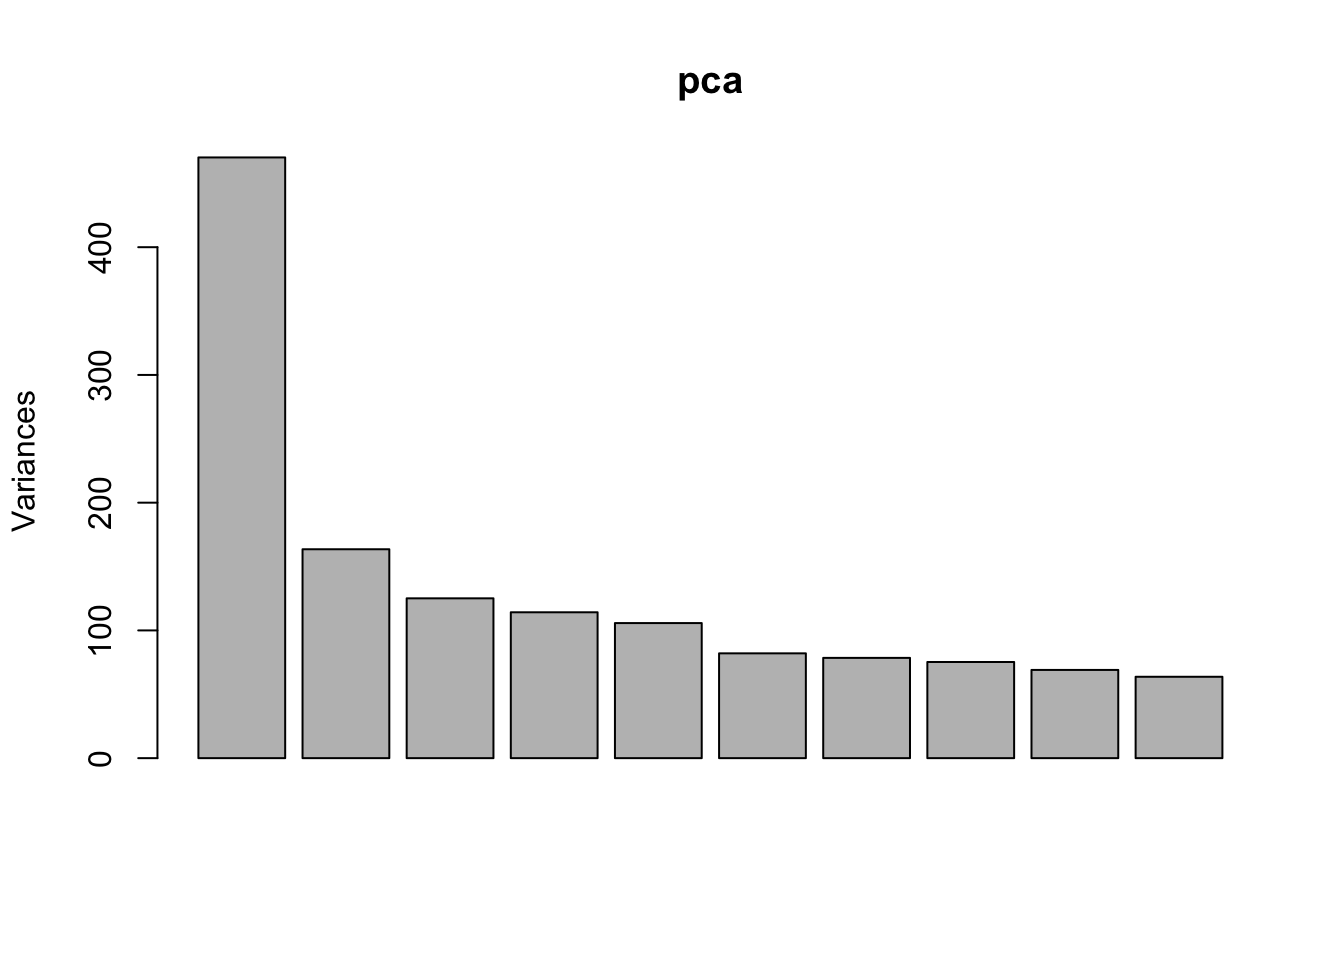
\includegraphics{NBDA_project_files/figure-latex/pca-1.pdf}
\caption{Variance explained by the first 10 components}
\end{figure}

\begin{Shaded}
\begin{Highlighting}[]
\CommentTok{\# draw PCA plot}
\NormalTok{group }\OtherTok{\textless{}{-}} \FunctionTok{c}\NormalTok{(}\FunctionTok{rep}\NormalTok{(}\StringTok{"cadetblue1"}\NormalTok{,}\DecValTok{18}\NormalTok{), }\FunctionTok{rep}\NormalTok{(}\StringTok{"red"}\NormalTok{,}\DecValTok{18}\NormalTok{), }\FunctionTok{rep}\NormalTok{(}\StringTok{"purple"}\NormalTok{,}\DecValTok{6}\NormalTok{) ) }\CommentTok{\# vector of colors based on the order of my data}
\FunctionTok{plot}\NormalTok{(pca}\SpecialCharTok{$}\NormalTok{x[,}\DecValTok{1}\NormalTok{], pca}\SpecialCharTok{$}\NormalTok{x[,}\DecValTok{2}\NormalTok{], }\AttributeTok{xlab=}\StringTok{"PCA1"}\NormalTok{, }\AttributeTok{ylab=}\StringTok{"PCA2"}\NormalTok{, }\AttributeTok{main=}\StringTok{"PCA for components 1 and 2"}\NormalTok{, }\AttributeTok{type=}\StringTok{"p"}\NormalTok{, }\AttributeTok{pch=}\DecValTok{10}\NormalTok{, }\AttributeTok{col=}\NormalTok{group)}
\FunctionTok{text}\NormalTok{(pca}\SpecialCharTok{$}\NormalTok{x[,}\DecValTok{1}\NormalTok{], pca}\SpecialCharTok{$}\NormalTok{x[,}\DecValTok{2}\NormalTok{], }\FunctionTok{rownames}\NormalTok{(pca}\SpecialCharTok{$}\NormalTok{data), }\AttributeTok{cex=}\FloatTok{0.75}\NormalTok{)}
\end{Highlighting}
\end{Shaded}

\includegraphics{NBDA_project_files/figure-latex/unnamed-chunk-7-1.pdf}

The vector group used in the PCA plot is based on the data. The samples
corresponding to the colors are the following:

\begin{itemize}
\item
  \textbf{Light blue}: reduction mammoplasty (RM) breast epithelium
  samples
\item
  \textbf{Red}: histologically normal (HN) epithelial samples from
  breast cancer patient
\item
  \textbf{Purple}: histologically normal breast epithelium (NlEpi) from
  prophylactic mastectomy patient samples
\end{itemize}

Let's try to explore an interactive PCA plot.

\begin{Shaded}
\begin{Highlighting}[]
\NormalTok{components}\OtherTok{\textless{}{-}}\NormalTok{pca[[}\StringTok{"x"}\NormalTok{]]}
\NormalTok{components}\OtherTok{\textless{}{-}}\FunctionTok{data.frame}\NormalTok{(components)}
\NormalTok{type}\OtherTok{\textless{}{-}}\FunctionTok{c}\NormalTok{(}\FunctionTok{rep}\NormalTok{(}\StringTok{"RM"}\NormalTok{, }\DecValTok{18}\NormalTok{), }\FunctionTok{rep}\NormalTok{(}\StringTok{"HN"}\NormalTok{,}\DecValTok{18}\NormalTok{), }\FunctionTok{rep}\NormalTok{(}\StringTok{"NlEpi"}\NormalTok{,}\DecValTok{6}\NormalTok{))}
\NormalTok{components}\OtherTok{\textless{}{-}}\FunctionTok{cbind}\NormalTok{(components, type )}

\NormalTok{fig }\OtherTok{\textless{}{-}} \FunctionTok{plot\_ly}\NormalTok{(components, }\AttributeTok{x=}\SpecialCharTok{\textasciitilde{}}\NormalTok{PC1, }\AttributeTok{y=}\SpecialCharTok{\textasciitilde{}}\NormalTok{PC2, }
               \AttributeTok{color=}\NormalTok{type,}\AttributeTok{colors=}\FunctionTok{c}\NormalTok{(}\StringTok{\textquotesingle{}cadetblue1\textquotesingle{}}\NormalTok{, }\StringTok{\textquotesingle{}red\textquotesingle{}}\NormalTok{,}\StringTok{\textquotesingle{}purple\textquotesingle{}}\NormalTok{), }
               \AttributeTok{type=}\StringTok{\textquotesingle{}scatter\textquotesingle{}}\NormalTok{,}\AttributeTok{mode=}\StringTok{\textquotesingle{}markers\textquotesingle{}}\NormalTok{)}
\NormalTok{fig}
\end{Highlighting}
\end{Shaded}

\begin{Shaded}
\begin{Highlighting}[]
\NormalTok{fig2 }\OtherTok{\textless{}{-}} \FunctionTok{plot\_ly}\NormalTok{(components, }\AttributeTok{x=}\SpecialCharTok{\textasciitilde{}}\NormalTok{PC1, }\AttributeTok{y=}\SpecialCharTok{\textasciitilde{}}\NormalTok{PC2, }\AttributeTok{z=}\SpecialCharTok{\textasciitilde{}}\NormalTok{PC3, }
                \AttributeTok{color=}\NormalTok{type, }\AttributeTok{colors=}\FunctionTok{c}\NormalTok{(}\StringTok{\textquotesingle{}cadetblue1\textquotesingle{}}\NormalTok{, }\StringTok{\textquotesingle{}red\textquotesingle{}}\NormalTok{,}\StringTok{\textquotesingle{}purple\textquotesingle{}}\NormalTok{),}
                \AttributeTok{mode=}\StringTok{\textquotesingle{}markers\textquotesingle{}}\NormalTok{, }\AttributeTok{marker =} \FunctionTok{list}\NormalTok{(}\AttributeTok{size =} \DecValTok{4}\NormalTok{))}
\NormalTok{fig2}
\end{Highlighting}
\end{Shaded}

\begin{Shaded}
\begin{Highlighting}[]
\NormalTok{fig3 }\OtherTok{\textless{}{-}} \FunctionTok{plot\_ly}\NormalTok{(components, }\AttributeTok{x=}\SpecialCharTok{\textasciitilde{}}\NormalTok{PC1, }\AttributeTok{y=}\SpecialCharTok{\textasciitilde{}}\NormalTok{PC3, }
                \AttributeTok{color=}\NormalTok{type, }\AttributeTok{colors=}\FunctionTok{c}\NormalTok{(}\StringTok{\textquotesingle{}cadetblue1\textquotesingle{}}\NormalTok{, }\StringTok{\textquotesingle{}red\textquotesingle{}}\NormalTok{,}\StringTok{\textquotesingle{}purple\textquotesingle{}}\NormalTok{),}
                \AttributeTok{type=}\StringTok{\textquotesingle{}scatter\textquotesingle{}}\NormalTok{,}\AttributeTok{mode=}\StringTok{\textquotesingle{}markers\textquotesingle{}}\NormalTok{)}
\NormalTok{fig3}
\end{Highlighting}
\end{Shaded}

\subsection{UMAP}\label{umap}

\begin{Shaded}
\begin{Highlighting}[]
\NormalTok{umap\_data }\OtherTok{\textless{}{-}}\NormalTok{ umap}\SpecialCharTok{::}\FunctionTok{umap}\NormalTok{(}\FunctionTok{t}\NormalTok{(normalized.log.ex), }
                        \AttributeTok{n\_neighbors =} \FunctionTok{sqrt}\NormalTok{(}\FunctionTok{dim}\NormalTok{(}\FunctionTok{t}\NormalTok{(normalized.log.ex))[}\DecValTok{1}\NormalTok{]),}\CommentTok{\#or the square root of the rows }
                        \AttributeTok{min\_dist =} \FloatTok{0.1}\NormalTok{,         }
                        \AttributeTok{metric =} \StringTok{"euclidean"}\NormalTok{,    }\CommentTok{\#you can change it}
                        \AttributeTok{n\_components =} \DecValTok{2}\NormalTok{) }\CommentTok{\#used the default ones! }

\NormalTok{umap\_df }\OtherTok{\textless{}{-}} \FunctionTok{data.frame}\NormalTok{(umap\_data}\SpecialCharTok{$}\NormalTok{layout) }\SpecialCharTok{\%\textgreater{}\%}\NormalTok{ tibble}\SpecialCharTok{::}\FunctionTok{rownames\_to\_column}\NormalTok{(}\StringTok{\textquotesingle{}Samples\textquotesingle{}}\NormalTok{)}
\NormalTok{umap\_df}\SpecialCharTok{$}\NormalTok{type}\OtherTok{\textless{}{-}}\FunctionTok{c}\NormalTok{(}\FunctionTok{rep}\NormalTok{(}\StringTok{"RM"}\NormalTok{, }\DecValTok{18}\NormalTok{), }\FunctionTok{rep}\NormalTok{(}\StringTok{"HN"}\NormalTok{,}\DecValTok{18}\NormalTok{), }\FunctionTok{rep}\NormalTok{(}\StringTok{"NlEpi"}\NormalTok{,}\DecValTok{6}\NormalTok{))}

\FunctionTok{library}\NormalTok{(plotly)}

\NormalTok{figUmap }\OtherTok{\textless{}{-}} \FunctionTok{plot\_ly}\NormalTok{(umap\_df, }
                 \AttributeTok{x =} \SpecialCharTok{\textasciitilde{}}\NormalTok{X1, }\AttributeTok{y =} \SpecialCharTok{\textasciitilde{}}\NormalTok{X2, }\AttributeTok{color =}\NormalTok{ umap\_df}\SpecialCharTok{$}\NormalTok{type,}
                 \AttributeTok{colors =} \FunctionTok{c}\NormalTok{(}\StringTok{\textquotesingle{}cadetblue1\textquotesingle{}}\NormalTok{, }\StringTok{\textquotesingle{}red\textquotesingle{}}\NormalTok{,}\StringTok{\textquotesingle{}purple\textquotesingle{}}\NormalTok{),   }
                 \AttributeTok{mode =} \StringTok{\textquotesingle{}markers\textquotesingle{}}\NormalTok{,}
                 \AttributeTok{size=}\DecValTok{1}\NormalTok{)}

\CommentTok{\# Display the 2D scatter plot}
\NormalTok{figUmap}
\end{Highlighting}
\end{Shaded}

\begin{verbatim}
## No trace type specified:
##   Based on info supplied, a 'scatter' trace seems appropriate.
##   Read more about this trace type -> https://plotly.com/r/reference/#scatter
\end{verbatim}

\begin{Shaded}
\begin{Highlighting}[]
\NormalTok{umap\_data\_3D }\OtherTok{\textless{}{-}}\NormalTok{ umap}\SpecialCharTok{::}\FunctionTok{umap}\NormalTok{(}\FunctionTok{t}\NormalTok{(normalized.log.ex), }
                        \AttributeTok{n\_neighbors =} \FunctionTok{sqrt}\NormalTok{(}\FunctionTok{dim}\NormalTok{(}\FunctionTok{t}\NormalTok{(normalized.log.ex))[}\DecValTok{1}\NormalTok{]),}
                      \CommentTok{\#or the square root of the rows, provato anche con 5 fa pena, anche 15 abbastanza pena  }
                        \AttributeTok{min\_dist =} \FloatTok{0.1}\NormalTok{,         }
                        \AttributeTok{metric =} \StringTok{"euclidean"}\NormalTok{,    }\CommentTok{\#you can change it}
                        \AttributeTok{n\_components =} \DecValTok{3}\NormalTok{) }\CommentTok{\#used the default ones! }

\NormalTok{umap\_df\_3D }\OtherTok{\textless{}{-}} \FunctionTok{data.frame}\NormalTok{(umap\_data\_3D}\SpecialCharTok{$}\NormalTok{layout) }\SpecialCharTok{\%\textgreater{}\%}\NormalTok{ tibble}\SpecialCharTok{::}\FunctionTok{rownames\_to\_column}\NormalTok{(}\StringTok{\textquotesingle{}Samples\textquotesingle{}}\NormalTok{)}
\NormalTok{umap\_df\_3D}\SpecialCharTok{$}\NormalTok{type}\OtherTok{\textless{}{-}}\FunctionTok{c}\NormalTok{(}\FunctionTok{rep}\NormalTok{(}\StringTok{"RM"}\NormalTok{, }\DecValTok{18}\NormalTok{), }\FunctionTok{rep}\NormalTok{(}\StringTok{"HN"}\NormalTok{,}\DecValTok{18}\NormalTok{), }\FunctionTok{rep}\NormalTok{(}\StringTok{"NlEpi"}\NormalTok{,}\DecValTok{6}\NormalTok{))}

\NormalTok{figUmap\_3D }\OtherTok{\textless{}{-}} \FunctionTok{plot\_ly}\NormalTok{(umap\_df\_3D, }
                 \AttributeTok{x =} \SpecialCharTok{\textasciitilde{}}\NormalTok{X1, }\AttributeTok{y =} \SpecialCharTok{\textasciitilde{}}\NormalTok{X2, }\AttributeTok{z=}\SpecialCharTok{\textasciitilde{}}\NormalTok{X3, }\AttributeTok{color =}\NormalTok{ umap\_df\_3D}\SpecialCharTok{$}\NormalTok{type,}
                 \AttributeTok{colors =} \FunctionTok{c}\NormalTok{(}\StringTok{\textquotesingle{}cadetblue1\textquotesingle{}}\NormalTok{, }\StringTok{\textquotesingle{}red\textquotesingle{}}\NormalTok{,}\StringTok{\textquotesingle{}purple\textquotesingle{}}\NormalTok{),   }
                 \AttributeTok{mode =} \StringTok{\textquotesingle{}markers\textquotesingle{}}\NormalTok{,}
                 \AttributeTok{size=}\DecValTok{1}\NormalTok{) }\SpecialCharTok{\%\textgreater{}\%} \FunctionTok{layout}\NormalTok{(}\AttributeTok{title =} \StringTok{\textquotesingle{}Umap 1 control{-}tumors 3D\textquotesingle{}}\NormalTok{)}

\CommentTok{\# Display the 2D scatter plot}
\NormalTok{figUmap\_3D}
\end{Highlighting}
\end{Shaded}

\begin{verbatim}
## No trace type specified:
##   Based on info supplied, a 'scatter3d' trace seems appropriate.
##   Read more about this trace type -> https://plotly.com/r/reference/#scatter3d
\end{verbatim}

```

\end{document}
